\documentclass[11pt]{article}
\usepackage[a4paper,margin=25mm]{geometry}
\usepackage[T1]{fontenc}
\usepackage[utf8]{inputenc}
\usepackage{lmodern,microtype}
\usepackage{amsmath,amssymb,amsthm,mathtools}
\usepackage{booktabs,array,enumitem}
\usepackage{xcolor}
\usepackage{pgfplots}
\pgfplotsset{compat=1.18}
\usepackage{needspace}
\usepackage[colorlinks=true,linkcolor=blue!45!black,citecolor=blue!45!black,urlcolor=blue!45!black]{hyperref}
\hypersetup{pdftitle={QK Feature Pairs and Interaction Terms in Attention Outputs},pdfauthor={FRA project},pdfsubject={Exact score interactions and constructive output-interaction theorems}}
\usepackage[nameinlink,noabbrev]{cleveref}
\usepackage{fancyhdr}
\pagestyle{fancy}
\fancyhf{}
\fancyhead[L]{\small QK feature pairs and activation interactions}
\fancyhead[R]{\small Technical note}
\fancyfoot[C]{\thepage}
\setlength{\headheight}{14pt}
\setlength{\parskip}{4pt}
\setlength{\parindent}{0pt}
\setlist{nosep,leftmargin=1.6em,topsep=5pt}
\setlength{\emergencystretch}{1.5em}
\newcommand{\R}{\mathbb{R}}
\newcommand{\E}{\mathbb{E}}
\newcommand{\softmax}{\operatorname{softmax}}
\newcommand{\logit}{\operatorname{logit}}
\newcommand{\ip}[2]{\langle #1,#2\rangle}
\newcommand{\norm}[1]{\lVert #1\rVert}
\newcommand{\QK}{\mathrm{QK}}
\newcommand{\OV}{\mathrm{OV}}
\newcommand{\pairdiff}{\Delta_{AB}}
\theoremstyle{plain}
\newtheorem{proposition}{Proposition}
\newtheorem{theorem}[proposition]{Theorem}
\newtheorem{corollary}[proposition]{Corollary}
\theoremstyle{definition}
\newtheorem{definition}[proposition]{Definition}
\theoremstyle{remark}
\newtheorem*{remark}{Remark}
\crefname{proposition}{Proposition}{Propositions}
\crefname{theorem}{Theorem}{Theorems}
\crefname{corollary}{Corollary}{Corollaries}
\crefname{definition}{Definition}{Definitions}

\title{QK Feature Pairs and Interaction Terms\\in Attention Outputs}
\author{FRA project --- technical note}
\date{10 September 2026}

\begin{document}
\maketitle
\thispagestyle{empty}

\begin{abstract}
Feature-resolved attention (FRA) expresses a query--key score as a sum of products of feature activations. We identify the precise sense in which these products are interactions. Under independent, fixed-background feature insertions, each QK pair contribution equals the corresponding two-player mixed difference of the pre-softmax score. For an isolated binary pair that changes one source score while all values and competing scores remain fixed, we prove a stronger result: the attention output is exactly a background activation plus a second-order interaction in a fixed direction. That direction is a contrast between transported values. This gives a constructive synthetic activation model and an exact pair-removal guarantee. We also give counterexamples to an unconditional output-level implication, show how multiple QK pairs can generate higher-order output interactions, and separate these statements from claims about SAE recovery or spontaneous learning.
\end{abstract}

\section{The question and the intervention convention}

The motivating question is whether meaningful interactions between residual-stream features are reflected in QK feature pairs. There are two directions to this question. One can start with a synthetic activation distribution containing a joint concept and ask whether a learned attention head uses its constituent features as a QK pair. Alternatively, one can start with a specified QK pair and derive the interactions in the resulting activations. This note establishes results in the second direction.

The objects must be distinguished. An \emph{input activation} is a vector supplied to the head. An \emph{attention score} is a scalar computed from two such vectors. An \emph{output activation} is the vector produced after softmax weighting and value transport. Below, reconstructed output activations mean outputs computed from specified feature contributions and attention weights; they do not mean that QK uniquely determines an SAE's reconstruction of its input.

\begin{definition}[Fixed-background two-feature interaction]\label{def:interaction}
Let $a,b\in\{0,1\}$ independently toggle two selected feature occurrences, and let $F(a,b)$ be a scalar or vector output. Define
\begin{equation}
\pairdiff F
 =F(1,1)-F(1,0)-F(0,1)+F(0,0).
\label{eq:delta}
\end{equation}
All other inputs and the background are held fixed across the four evaluations. For vector outputs the difference is taken componentwise.
\end{definition}

This is the unnormalised two-player Harsanyi, or M\"obius, interaction. It is the elementary mixed difference used in Shapley-style interaction attribution; it is not an ordinary Shapley value. For the two-player game, the ordinary Shapley attribution to $A$ is
\begin{equation}
\phi_A=F(1,0)-F(0,0)+\tfrac12\pairdiff F,
\label{eq:shapley}
\end{equation}
and likewise for $B$. Thus individual Shapley values redistribute the interaction between its participants. With more players, interaction indices can average differences over backgrounds or redistribute higher-order terms; their conventions must be specified separately~\cite{sundararajan2020}. No particular normalisation for a full SHAP interaction matrix is assumed here.

The players are \emph{feature occurrences at positions}. A feature of identity $i$ at position $q$ and a feature of the same identity at position $k\ne q$ are still two players. ``Second order'' refers to two players, not matrix rank. Off-diagonal QK entries couple different feature identities, but diagonality is not the boundary between interactions and non-interactions.

\section{A QK pair is exactly a score interaction}

Use column vectors, and consider one head at fixed query and source positions $q,k$. Let $x_q,x_k\in\R^d$ be the vectors entering the linear Q/K maps. Set
\begin{equation}
 M=\frac{W_Q^\top W_K}{\sqrt{d_h}},
 \qquad s_{qk}=x_q^\top Mx_k.
\label{eq:score}
\end{equation}
Query/key biases only add constant or single-player terms and can be absorbed into the background below. A fixed positional rotation can likewise be included in a position-dependent $M_{qk}$.

Let $d_i,d_j$ be feature directions and $u,v$ their selected activation amplitudes. Define independent insertions
\begin{equation}
 x_q(a)=x_q^{\mathrm{bg}}+a\,u d_i,
 \qquad
 x_k(b)=x_k^{\mathrm{bg}}+b\,v d_j.
\label{eq:insertions}
\end{equation}
The directions can be ground truth or SAE decoder directions. If an SAE decomposition has a residual error, that error is included in the fixed background. We do not re-encode the four intervened vectors.

\begin{proposition}[Exact score identity]\label{prop:score}
Under \cref{eq:insertions}, the score has the expansion
\begin{equation}
 s_{qk}(a,b)=s_{\mathrm{bg}}+\alpha a+\beta b+\gamma ab,
 \qquad
 \gamma=uv\,d_i^\top M d_j.
\label{eq:score-expansion}
\end{equation}
Consequently,
\begin{equation}
 \boxed{\pairdiff s_{qk}=uv\,d_i^\top M d_j
       =\text{the selected FRA QK pair contribution}.}
\label{eq:score-identity}
\end{equation}
\end{proposition}
\begin{proof}
Expand \cref{eq:score} after substituting \cref{eq:insertions}. The constant term is $(x_q^{\mathrm{bg}})^\top Mx_k^{\mathrm{bg}}$, the single-player terms are $u d_i^\top Mx_k^{\mathrm{bg}}$ and $v(x_q^{\mathrm{bg}})^\top Md_j$, and the product term is $uv d_i^\top Md_j$. Applying \cref{eq:delta} cancels the constant and single-player terms.
\end{proof}

The coefficient $d_i^\top Md_j$ is not by itself the contribution on an example: the amplitudes $u,v$ also matter. A nonzero coefficient produces a nonzero score interaction when both selected amplitudes are nonzero.

\paragraph{Scope of the identity.}
This proposition concerns the pre-softmax \emph{bilinear score}. For a normalised transformer, $x$ denotes the post-normalisation input to Q/K. Recomputing normalisation after editing a pre-normalisation residual vector can change the background and invalidate \cref{eq:insertions}. A nonlinear score cap also need not preserve \cref{eq:score-identity} for the capped score. Finally, independently inserting features is an intervention convention: if a data generator also updates a compound feature whenever $a$ or $b$ changes, its four data examples define a different game.

\section{An isolated pair gives an exact output interaction}

The score identity holds without assumptions about values or competing keys. An output theorem needs both. Let $\mathcal K$ be a fixed finite set of at least two unmasked sources. Write $v_t\in\R^d$ for the source's value \emph{after} the output projection, so the head writes
\begin{equation}
 y=\sum_{t\in\mathcal K}p_t v_t,
 \qquad p=\softmax(s).
\label{eq:head-output}
\end{equation}
This is the usual QK/OV separation~\cite{elhage2021}. We use the logistic sigmoid $\sigma(z)=(1+e^{-z})^{-1}$ and its inverse $\logit(p)=\log[p/(1-p)]$.

\begin{theorem}[Fixed-value, single-source pair]\label{thm:output}
Suppose the only change to the score vector is
\begin{equation}
 s_1(a,b)=s_1^0+\gamma ab,
 \qquad s_t(a,b)=s_t^0\quad(t\ne1),
\label{eq:isolated-score}
\end{equation}
and all $v_t$ remain fixed. Assume finite scores, and define
\begin{equation}
 p=p_1(0,0),\qquad
 \bar v_- =\frac{\sum_{t\ne1}p_t(0,0)v_t}{1-p},\qquad
 p_\gamma=\sigma\!\left(\logit(p)+\gamma\right).
\label{eq:competitors}
\end{equation}
Then $0<p<1$, and the head output is exactly
\begin{equation}
 \boxed{y(a,b)=y_0+abD_{AB},\qquad
 D_{AB}=(p_\gamma-p)(v_1-\bar v_-),}
\label{eq:output-interaction}
\end{equation}
where $y_0=pv_1+(1-p)\bar v_-$. In particular, $\pairdiff y=D_{AB}$, which is nonzero if and only if $\gamma\ne0$ and $v_1\ne\bar v_-$.
\end{theorem}

\begin{proof}
The relative weights of sources other than $1$ are unchanged, so their conditional mean value is always $\bar v_-$. The selected source has attention odds
\[
 \frac{p_1(a,b)}{1-p_1(a,b)}
   =\frac{p}{1-p}\exp(\gamma ab).
\]
Since $ab\in\{0,1\}$, its probability is $p_1(a,b)=p+ab(p_\gamma-p)$. Substitution into $y=p_1v_1+(1-p_1)\bar v_-$ gives \cref{eq:output-interaction}. The sigmoid is strictly increasing at finite arguments, hence $p_\gamma=p$ if and only if $\gamma=0$.
\end{proof}

The interaction direction is a \emph{value contrast}. It need not equal either input feature direction. QK determines how strongly the source is selected, while OV and the alternatives determine what activation that selection changes. For a scalar readout $L=\ell^\top y$, the interaction is nonzero only if $\ell^\top(v_1-\bar v_-)\ne0$.

\begin{corollary}[Exact pair removal]\label{cor:removal}
Under \cref{thm:output}, subtracting $\gamma ab$ from the selected score restores $y_0$ for all four feature conditions. If other contributions to the reconstructed activation have the fixed additive form $R_0+aU_A+bU_B$, they remain unchanged, and
\[
 R_0+aU_A+bU_B+y_0+abD_{AB}
 \quad\longmapsto\quad
 R_0+aU_A+bU_B+y_0.
\]
\end{corollary}
This is an exact intervention result for the stated construction, not a claim of superiority over all residual-steering baselines. Nor does cancelling the score term mean setting its attention probability to zero: it restores the baseline attention distribution.

\subsection{The two-source example}
Take scores $\gamma ab$ and $0$. Then $p=1/2$ and
\begin{equation}
 y(a,b)=\frac{v_1+v_0}{2}
   +ab\left(\sigma(\gamma)-\frac12\right)(v_1-v_0).
\label{eq:two-source}
\end{equation}
With $v_1=d$, $v_0=-d$, this reduces to
\begin{equation}
 \boxed{y(a,b)=ab\,\tanh(\gamma/2)\,d.}
\label{eq:opposite-values}
\end{equation}
For example, $\gamma=\log 3$ gives a write of $d/2$ in the joint condition and zero in the other three conditions. The opposite values remove a constant background; arbitrary fixed values give the same interaction plus the background in \cref{eq:two-source}.

\begin{figure}[htbp]
\centering
\begin{minipage}[c]{0.40\textwidth}
\centering
\renewcommand{\arraystretch}{1.3}
\begin{tabular}{cccc}
\toprule
$a$ & $b$ & $p_1$ & $y$ \\
\midrule
0 & 0 & $1/2$ & $0$ \\
1 & 0 & $1/2$ & $0$ \\
0 & 1 & $1/2$ & $0$ \\
1 & 1 & $3/4$ & $d/2$ \\
\bottomrule
\end{tabular}
\end{minipage}\hfill
\begin{minipage}[c]{0.56\textwidth}
\centering
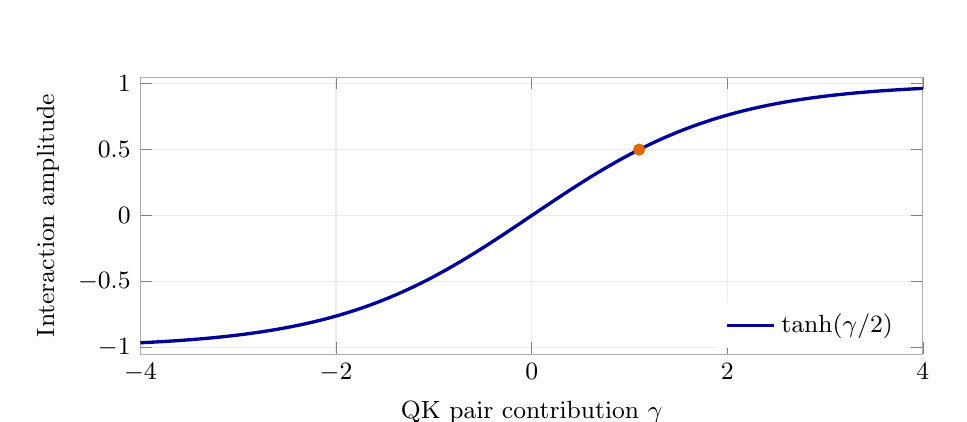
\begin{tikzpicture}
\begin{axis}[
 width=0.95\linewidth,height=5.1cm,
 xlabel={QK pair contribution $\gamma$},
 ylabel={Interaction amplitude},
 xmin=-4,xmax=4,ymin=-1.05,ymax=1.05,
 xtick={-4,-2,0,2,4},ytick={-1,-0.5,0,0.5,1},
 tick label style={font=\small},label style={font=\small},
 grid=major,grid style={gray!15},axis line style={gray!65},
 legend style={draw=none,font=\small,at={(0.98,0.02)},anchor=south east},
 ]
\addplot[very thick,blue!60!black,domain=-4:4,samples=121]{tanh(x/2)};
\addlegendentry{$\tanh(\gamma/2)$}
\addplot[only marks,mark=*,mark size=2pt,orange!85!black] coordinates {(1.098612288668,0.5)};
\end{axis}
\end{tikzpicture}
\end{minipage}
\caption{Exact analytic output interaction for an isolated binary QK pair with $v_1=d$ and $v_0=-d$. Left: the four conditions at $\gamma=\log3$. Right: the coefficient of $ab\,d$ as the QK pair strength varies; the dot marks the tabulated example. These are consequences of \cref{eq:opposite-values}, not empirical training results.}
\label{fig:gain}
\end{figure}

\section{A synthetic activation model generated by a QK pair}

The two-source example can be realised by an ordinary linear-projection attention head. Choose orthonormal input directions $e_A,e_B,e_S,e_R$, and an output direction $d$ independent of them. Supply
\begin{equation}
 x_q=a e_A,\qquad x_1=b e_B+e_S,\qquad x_0=e_R,
\label{eq:synthetic-input}
\end{equation}
with a fixed mask allowing the query to attend to sources $1$ and $0$. Use head dimension one, no normalisation or score cap, and
\begin{equation}
 W_Q=\gamma e_A^\top,\quad W_K=e_B^\top,
 \quad W_V=e_S^\top-e_R^\top,\quad W_O=d.
\label{eq:synthetic-weights}
\end{equation}
Then the scores are $\gamma ab,0$, the projected values are $d,-d$, and the residual output at the query is
\begin{equation}
 x'_q=a e_A+ab\,\tanh(\gamma/2)d.
\label{eq:synthetic-output}
\end{equation}
The source's individual feature is present as $b e_B$ in its input activation. Local readouts of the constituent input features remain available. Additional additive output channels may be included if both individual effects should also appear explicitly in the query's output. In all cases, a score-only pair edit leaves those specified input and additive channels unchanged.

This gives a data generator with a known computational origin for its joint concept. Sample $a,b$, construct \cref{eq:synthetic-input}, and generate output activations using \cref{eq:synthetic-output}. The interaction strength is $\lambda=\tanh(\gamma/2)$, with a zero-interaction control at $\gamma=0$. The scale of $d$ independently controls the size of the resulting activation write. Nothing in this construction requires an SAE; an SAE is subsequently an object to evaluate against the known feature directions and activations.

\subsection{Anchored interaction versus a statistically pure interaction}

The coefficient of $ab$ is an exact interaction relative to the zero-feature baseline in \cref{def:interaction}. It is not exclusively interaction variance under a sampling distribution. If $a,b$ are independent Bernoulli variables with means $p_A,p_B$, then
\begin{align}
 abD_{AB}={}&(a-p_A)(b-p_B)D_{AB}
       +p_B(a-p_A)D_{AB}\notag\\
       &+p_A(b-p_B)D_{AB}+p_Ap_BD_{AB}.
\label{eq:anova}
\end{align}
The first term is the functional-ANOVA interaction: its conditional expectation given either feature is zero, and it is orthogonal to all additive single-feature functions~\cite{lengerich2020}. Its expected squared norm is
\[
 p_A(1-p_A)p_B(1-p_B)\norm{D_{AB}}^2.
\]
Thus sweeping $\gamma$ in the raw conjunction construction also changes the mean and marginal effects. A control that varies only statistically pure interaction strength must compensate the other terms in \cref{eq:anova}, for example through known additive channels. The two conventions answer different questions; neither should be substituted silently for the other.

\section{Why the unrestricted implication fails}

\paragraph{Equal values and common score shifts.}
If every source has the same value, the output is constant for every attention pattern, even when individual scores have nonzero QK interactions. Similarly, adding the same $\gamma ab$ to every score leaves the softmax unchanged. An edge's absolute score interaction alone is insufficient.

\paragraph{Main effects can cancel an output interaction.}
The isolated-pair assumption in \cref{eq:isolated-score} matters even with two distinct fixed values. Let $v_1=1,v_0=0$ and choose the four attention probabilities as
\[
 (p_{00},p_{10},p_{01},p_{11})=(0.2,0.3,0.4,0.5).
\]
They have $\pairdiff y=0$. Nevertheless, the corresponding source-minus-reference scores $s_{ab}=\logit(p_{ab})$ have
\begin{equation}
 \pairdiff s=\log(7/8)\ne0.
\label{eq:cancellation}
\end{equation}
These four scores are realised by \cref{eq:score-expansion} with
$s_{\mathrm{bg}}=\log(1/4)$, $\alpha=\log(12/7)$, $\beta=\log(8/3)$, and $\gamma=\log(7/8)$. A nonzero QK cross term therefore need not survive as a nonzero output mixed difference when score main effects also vary.

\paragraph{The converse also fails.}
For $s(a,b)=a+b$ and the same two values, $\pairdiff s=0$, but
\[
 \pairdiff y=\sigma(2)-2\sigma(1)+\tfrac12\ne0.
\]
The softmax nonlinearity can create an output interaction from additive score effects. If a feature also changes the values, a joint output effect can instead arise from a query-dependent attention weight multiplying a feature-dependent value. This is not necessarily a QK interaction between those same constituent features.

\paragraph{Continuous amplitudes.}
For real-valued $a,b$, the opposite-value example gives $y=\tanh(\gamma ab/2)d$, rather than an exactly bilinear activation map. For small $|\gamma ab|$,
\[
 y=\left(\frac{\gamma ab}{2}-\frac{\gamma^3a^3b^3}{24}
       +O((\gamma ab)^5)\right)d.
\]
Higher polynomial degree in the same two variables is not a higher interaction order in the coalition sense. Binary gating is what makes the exact $abD_{AB}$ representation possible over the entire four-point domain.

\paragraph{Several pairs can generate higher-order interactions.}
Let $a,b,c,e\in\{0,1\}$, keep opposite values $d,-d$, and use scores $\gamma ab+\eta ce$ and zero. Define $T(t)=\tanh(t/2)$. The output is exactly
\begin{equation}
 y=\left[T(\gamma)ab+T(\eta)ce
  +\{T(\gamma+\eta)-T(\gamma)-T(\eta)\}abce\right]d.
\label{eq:four-way}
\end{equation}
The last coefficient is generally nonzero: two pairwise score terms create a four-player output interaction. For $\gamma=\eta=\log3$, this becomes $(\tfrac12 ab+\tfrac12 ce-\tfrac15 abce)d$. Hence a head containing many FRA pairs does not generally yield an additive dictionary of independent second-order output terms.

For a general fixed-value head, the local differential makes the role of competition explicit:
\begin{equation}
 \delta y=\sum_t p_t\,\delta s_t\,(v_t-y).
\label{eq:jacobian}
\end{equation}
This is a first-order statement, whereas \cref{thm:output} is finite and exact. Neither statement guarantees an effect on a downstream task if its readout is insensitive to the resulting direction.

\section{What this establishes for FRA and SAEs}

There are three separate statements:
\begin{enumerate}
\item \textbf{Score attribution.} Under fixed-background feature insertions, a FRA QK pair contribution is exactly a two-player interaction of the bilinear score.
\item \textbf{Constructive activation generation.} An isolated pair with fixed competing scores and a nonzero value contrast produces an exact second-order output activation term. Cancelling that score pair removes this term and preserves the explicitly independent additive channels.
\item \textbf{Recovery by learning.} Whether an SAE recovers the relevant features, or a newly trained head rediscovers the generating QK pair, is not proved by either result above.
\end{enumerate}

An SAE trained on outputs such as \cref{eq:synthetic-output} may represent $ab\,d$ as a single feature with activation $ab$. That is compatible with its generation by a QK pair: interaction order in the underlying variables is different from the number of features in an output dictionary. Sparsity, reconstruction quality, and the geometry of $d$ relative to other directions affect recovery and require separate analysis.

Nor is the generating mechanism uniquely determined by the activation distribution. If the query input already supplies a compound feature $c=ab$, a score $\theta a b$ can be replaced by $\theta c\cdot1$, using a constant source-marker feature, while retaining a reference score of zero. Both heads have the same scores and outputs on that distribution, but only one uses the constituent $A\times B$ cell. Full feature recovery does not resolve this functional dependence.

For a synthetic study, the constructive model supplies ground truth rather than an automatic learning guarantee. One can compare an additive control with planted interactions, analyse the same learned head in ground-truth and SAE bases, and measure whether candidate pair edits remove the known output mixed difference while preserving the single-feature effects. A larger study can vary interaction co-occurrence, value contrasts, feature overlap, and head capacity. Claims of improved intervention performance would additionally require matched DoM and single-feature baselines; none follows from the algebra alone.

\begin{thebibliography}{9}
\bibitem{sundararajan2020}
M. Sundararajan, K. Dhamdhere, and A. Agarwal.
\newblock The Shapley Taylor Interaction Index.
\newblock In \emph{Proceedings of ICML}, PMLR 119:9259--9268, 2020.
\newblock \url{https://proceedings.mlr.press/v119/sundararajan20a.html}.

\bibitem{lengerich2020}
B. Lengerich, S. Tan, C.-H. Chang, G. Hooker, and R. Caruana.
\newblock Purifying Interaction Effects with the Functional ANOVA: An Efficient Algorithm for Recovering Identifiable Additive Models.
\newblock In \emph{Proceedings of AISTATS}, PMLR 108:2402--2412, 2020.
\newblock \url{https://proceedings.mlr.press/v108/lengerich20a.html}.

\bibitem{elhage2021}
N. Elhage et al.
\newblock A Mathematical Framework for Transformer Circuits.
\newblock \emph{Transformer Circuits}, 2021.
\newblock \url{https://transformer-circuits.pub/2021/framework/index.html}.
\end{thebibliography}

\end{document}
